% latexmk -quiet -bibtex -aux-directory=AuxDirectory --output-directory=PDF -pdf -pdflatex="pdflatex -synctex=1 -interaction=nonstopmode" main.tex
\documentclass[12pt,a4paper]{article}%fleqn,leqno
\usepackage[utf8]{inputenc}
\usepackage[english,russian]{babel}
\usepackage{extsizes}
\usepackage[unicode, colorlinks=false, urlcolor=blue, pdfborder={0 0 0 [0 0]},bookmarks=false]{hyperref}
\usepackage{mathtext}
\usepackage[T2A]{fontenc}
\usepackage{alltt}
\usepackage{amsmath}
\usepackage{amsthm}
\usepackage{amssymb}
\usepackage{graphics}
\usepackage{graphicx}
\usepackage{fancyhdr}
\usepackage{caption}
\usepackage{indentfirst}
\usepackage{multirow}
\usepackage{hhline}
\usepackage{tabularx}
\usepackage{longtable}
\usepackage{multicol}
\usepackage{rotating}
\usepackage{sectsty}
\usepackage{titlesec}
\usepackage[dvipsnames, usenames]{color}
\usepackage{wrapfig}
\usepackage{pgf}
\usepackage{tikz}%pgfplots}
\usepackage{pgfplots}
%\usepackage{mathtools}

\usepackage{algorithm}
\usepackage[noend]{algpseudocode}

\makeatletter
\def\BState{\State\hskip-\ALG@thistlm}
\makeatother

\usepackage{subfigure}
\usepackage{units}
\usepackage{cmap}
\usepackage{setspace}
\usepackage{cite}
\usepackage[section,above,below]{placeins}
\usepackage{epstopdf} %for MikTex
\usepackage{float}
\usepackage{color}

\graphicspath{ {img/} }
\usepackage{pscyr}
\renewcommand{\rmdefault}{ftm}

\newcommand*{\mathcolor}{}
\def\mathcolor#1#{\mathcoloraux{#1}}
\newcommand*{\mathcoloraux}[3]{%
  \protect\leavevmode
  \begingroup
    \color#1{#2}#3%
  \endgroup
}
\newcommand{\fat}{\mathbf}

\newtheorem{theor}{Теорема}
\newtheorem{theorem}{Теорема}
\newtheorem{lemma}{Лемма}
\newtheorem{proposition}{Proposition}
\newtheorem{corollary}{Corollary}
\newtheorem{definition}{Определение}


\usepackage[left=2.5cm,right=1cm,top=2cm,bottom=2cm]{geometry}


\begin{document}
% \section{Введение}
%     Задачи оптимального управления сложного теплообмена в рассеивающей среде с отражающими границами представляют выскоий интерес для изучения в связи с инженерными приложениями. Существует естественный интерес к исследованию задач по сложному теплообмену ввиду слабой изученности данных моделей. Анализ данного физического процесса важен для предприятий металлургии, стекольного производства, теплоэнергетики, пищевой промышленности, медицине и других отраслей.

%     В настоящей работе рассматривается задача получения необходимой температуры в случае управления степенью черноты границы области. Существующие алгоритмы вычисления оптимального bang-bang управления разработаны главным образом для одномерных управлений, например, зависящих от времени. В данной работе оптимальное управление достигается посредством градиентного метода с проекцией. Доказана разрешимость задачи оптимального управления и приведена система оптимальности. Приведены результаты численных экспериментов.

\section{Формулировка исходной краевой задачи}
    Нормализованная стационарная модель, описывающая процесс теплопереноса через излучение и теплопроводность в области $\Omega \subset \mathbb{R}^2$ (см. \cite{OControl_1}), имеет следующий вид:
    \begin{equation}
        \label{initial}
        \begin{aligned}
            - a \Delta \theta + b \kappa_a(\theta ^ 3 | \theta | - \varphi) = 0,  \\
            - \alpha \Delta \varphi + \kappa_a (\varphi - \theta ^3 | \theta |) = 0.
        \end{aligned}
        % \qquad \text{в } \Omega.
    \end{equation}

    Здесь $\theta$ -- нормализованная температура, $\varphi$ -- нормализованная интенсивность излучения, усредненная по всем направлениям, $\kappa_a$ -- коэффициент поглощения. Константы $a, b, \alpha, \gamma, \beta$ описываются следующим образом:
    $$
    a = \frac{k}{\rho c_v}, \; b = \frac{4 \sigma n^2 T^3_{\text{max}}}{\rho c_v}, \; \alpha = \frac{1}{3\kappa -A \kappa_s}
    $$
    где $k$ -- теплопроводность, $c_v$ -- удельная теплоёмкость, $\rho$ -- плотность, $\sigma$ -- постоянная Стефана -- Больцмана, $n$ -- индекс рефракции, $T_{\text{max}}$ -- максимальная температура, $\kappa := \kappa_s + \kappa_a$ -- коэфициент полного взаимодействия, $\kappa_s$ -- коэфициент рассеяния. Коэфициент $A \in [-1,1]$ описывает анизотропию рассеивания, при чем случай $A=0$ отвечает изотропному рассеиванию.

    В работе рассмотрены следующие граничные условия на $\Gamma := \partial \Omega =\bar{\Gamma_0} \cup \bar{\Gamma_1} \cup \bar{\Gamma_2}$
    
    \begin{equation}
        \label{initial_boundary}
        \begin{aligned}
            \Gamma: \; a \partial_n \theta + \beta (\theta - \theta _b) = 0, \\
            \Gamma_0 \cup \Gamma_2: \; \alpha \partial_n \varphi + \gamma(\varphi - \theta_b ^4 ) = 0, \\
            \Gamma_1: \; \alpha \partial_n \varphi + u(\varphi - \theta_b ^4 ) = 0, \\
        \end{aligned}
    \end{equation}
    Функции $\gamma, \theta_b, \beta$ -- являются известными. Функция $u$ -- является неизвестной и характеризует отражательные свойства границы. Предполагается, что
    \begin{equation}
        \label{control_bounds}
        0 \leq u_1 \leq u \leq u_2,
    \end{equation}
    где $u_1$ и $u_2$ - заданные функции, накладывающие ограничение на значения функции $u$.
    
\section{Постановка обратной экстремальной задачи}

Основной целью данной работы является исседование исследование единственности и устойчивости решений задач оптимального управления для рассматриваемой модели. Эти задачи заключаются в минимизации некоторых функционалов качества, зависящих от переменных состояния и неизвестных функций (функций управления), удовлетворяющих уравнениям состояния \eqref{initial}--\eqref{control_bounds}. 

    В данной работе будет рассмотрен следующий функционал качества:
    \begin{equation}
        \label{quality}
        J = \frac{1}{2} \int_{\Gamma_2} (\theta - \theta_0)^2 d\Gamma \rightarrow \text{inf}.
    \end{equation}
    $\theta_0 \in L^2(\Gamma)$ - известна.


    Будем предполагать что модель удовлетворяет следующим условиям :

(i) $\beta, \gamma, u_1, u_2 \in L^\infty(\Gamma); \gamma \ge \gamma_0 > 0;\; 0 \le u_1 \le u_2;$

(ii) Функционал качества $J : H \times U_{ad} \rightarrow \mathbb{R}$ является слабо полунепрерывным снизу.

Здесь и далее пространство Соболева $W^s_2(\Omega)$ обозначено через $H^s(\Omega), \; s \ge 0$,

$(f, g)$ и $\|f\|$ обозначают скалярное произведение и норму в пространстве $L^2(\Omega)$.

Обозначим за $H = L^2(\Omega), V = H^1(\Omega), Y = V \times V $. Пространство $H$ отождествляем с пространством $H'$ так,  что $V \subset H = H' \subset V'$. Определим $(f,v)$ как значение функционала $f \in V'$ на элементе $v \in V$, совпадающее со скалярным произведением в $H$, если $f\in H$. Пространство $U = L^2(\Gamma)$ является пространством управлений. Множество допустимых управлений: $U_{ad} = \{u \in U, u_1 \le u \le u_2 \}$.

Пусть $v$ произвольный элемент множества $H^1(\Omega)$. Определим следующие операторы:

$$A_{1,2}\colon V \to V', \;\; F \colon V \times U \to V',$$
$$(A_1,\theta,v) = a( \nabla \theta, \nabla v ) + \int_\Gamma \beta \theta v d\Gamma, \;
(A_2 \varphi, v) = \alpha (\nabla \varphi,\nabla v) + \int_{\Gamma_0 \cup \Gamma_2} \gamma \varphi v d\Gamma,$$
$$(f,v) = \int_\Gamma \beta \theta_b v d\Gamma, \; \;
(g,v) = \int_{\Gamma_0 \cup \Gamma_2} \gamma \theta_b^4 v d\Gamma$$
$$(F(\varphi, u), v) = \int_{\Gamma_1} u (\varphi - \theta^4_b)v d\Gamma.$$

Пару $\{\theta, \varphi \}$ будем называть слабым решением для задачи (\ref{initial}--\ref{initial_boundary}) если
\begin{equation}
    \label{weak_operational}
    A_1 \theta + b \kappa_a (| \theta | \theta^3 - \varphi ) = f, A_2 \varphi + \kappa_a (\varphi - |\theta|\theta^3) + F(\varphi, u) = g.
\end{equation}

Задача оптимального управления параметром на границе состоит в минимизации функционала $
J(\theta, u)$, определенном на решениях системы \eqref{weak_operational}.
    Таким образом
    \begin{equation}
        \label{minimization_operational}
        J(\theta, u) \to \text{inf}, \; \{\theta, \varphi\} \text{ решение \eqref{weak_operational},   соответсвующее  функции } u \in U_{ad}.
    \end{equation}

    Пара $\{\hat{\theta}, \hat{\varphi} \}$ соответствующая минимуму $J(\theta, u)$, отвечающая функции $\hat{u}$ называется оптимальным состоянием. В таком случае $\hat{u}$ называется оптимальным управлением.


\section{Разрешимость задачи оптимального управления}
    Для доказательства разрешимости задачи \eqref{minimization_operational} нам необходимо также установить некоторые свойства начальной задачи (\ref{initial}, \ref{initial_boundary}, \ref{quality}).

    \begin{lemma}
    \label{SolvabilityLemma}

    Если условия (i)--(ii) выполняются, то для каждого $ u \in U_{ad} $ существует единственное слабое решение $\{\theta, \varphi \}$ для задачи (\ref{initial}--\ref{initial_boundary}), и следующие оценки верны:
    \begin{equation}
        \label{lemma_1}
     M_1 \le \theta \le M_2, \; M_1^4 \le \varphi \le M_2^4,
     \end{equation}

    \begin{equation}
    \label{lemma_2}
     \| \nabla \varphi \|^2 \le C.
     \end{equation}
    Здесь $M_1 = \text{ess inf } \theta_b, M_2 = \text{ess sup } \theta_b$, и константа $C > 0$ зависит исключительно от \\ $a, b, \alpha, \kappa_a, \|u\|_{L^\infty(\Gamma)}, \| \gamma \|_{L^\infty(\Gamma)}$ и области $\Omega$.
    \end{lemma}
    Доказательство присутствует в работе \cite{lemma_proof}.
    Основываясь на оценках \eqref{lemma_1} и \eqref{lemma_2} аналогично с \cite{theorem_2_proof} доказывается разрешимость задачи оптимального управления \eqref{minimization_operational}.

    \begin{theorem}
        Если условия (i)--(ii) выполняются, тогда существует хотя бы одно решение задачи \eqref{minimization_operational}.
    \end{theorem}

\section{Необходимые условия оптимальности}
\label{sec:optimality}
    Для получения условий оптимальности нам необходимо добавить слудеющее условие:

    (iii) Функционал $J : V \times U_{ad} \rightarrow \mathbb{R}$ дифференцируем по Фреше.

    Аналогично с \cite{theorem_2_proof} доказывается следующая теорема
    \begin{theorem}
        Пусть $\hat{y}=\{\hat{\theta},\hat{\varphi} \} \in Y, \hat{u} \in U_{ad}$ будет решением задачи оптимального управления \eqref{minimization_operational}. Тогда существует пара $(\lambda, p) \in \mathbb{R}_{+} \times Y \setminus \{0\}$
        такое, что тройка значений $(\hat{y}, \hat{u}, p)$, где $p = (p_1, p_2)$ удовлетворяет следующим равенствам
        \begin{equation}
        \label{therorem_2_eq1}
         A_1 p_1 + 4 \hat{\theta}^3 \kappa_a(b p_1 - p_2) = f_c, \;\; (f_c,v) = - \int_{\Gamma_2} (\theta - \theta_0) v d\Gamma,
        \end{equation}

        \begin{equation}
        \label{therorem_2_eq2}
        A_2 p_2 + \kappa_a (p_2-b p_1) = g_c(( p_2, \hat{u}),v), \; \; g_c(( p_2, \hat{u}),v) = - \int_{\Gamma_1} u p_2 v\Gamma,
        \end{equation}

        \begin{equation}
        \label{therorem_2_eq3}
        \int_{\Gamma_1} p_2 (\hat{\varphi} - \theta_b^4)(u-w) \leq 0, \; \; \forall w \in U_{ad}.
        \end{equation}

    \end{theorem}

    \begin{proof}

        Доказательство данной теоремы основывается на принципе множителей Лагранжа для гладких выпуклых задач минимизации, с ограничениями типа равенств.

        Перепишем уравнения \eqref{weak_operational} следующим образом:
        $$H(y,u) = 0,\;\; y = \{\theta,\varphi\} \in Y,$$
        где
        $$ H:Y \times U \to Y', $$
        $$H(y,u) =\{A_1 \theta + b \kappa_a (| \theta | \theta^3 - \varphi ) - f, A_2 \varphi + \kappa_a (\varphi - |\theta|\theta^3) + F(\varphi, u) - g \}.$$
        Заметим, что для всех $u \in U_{ad}$, отображение $y \to J(y) $ и $y \to H(y,u)$ непрерывно дифференцируемо в окрестности $\mathcal{O}(\hat{y})$ точки $\hat{y}$. Непрерывная дифференцируемость членов в $H$ следует из непрерывной дифференцируемости функции $t \in \mathbb{R} \to | t | t^3$, а также из непрерывности вложения  $V \subset L^6(\Omega)$.
        В дополнение, отображение $u \to H(y,u)$ непрерывно из $U \to Y'$ и афинно.

        Аналогично с \cite[Th.2]{theorem_2_proof}, мы можем доказать плотность множества
         $\text{Im}H_y'(\hat{y},b u)$
        а также условие $\text{codim}(\text{Im}H_y') < \infty$.

        Рассмотрим функцию Лагранжа
        $L(y,u,\lambda,p) = \lambda J(y) + (H(y,u),p),$
        где $\lambda \in \mathbb{R}_+$, $y,p \in Y$ , и $u \in U_{ad}$. согласно принципу Лагранжа (\cite[Ch.2 Th.1.5]{theorem_proof_18}) существует пара $(\lambda, p) \in (\mathbb{R}_+ \times Y ) /\ \{0,0\}$
        ($\lambda$ или $p$ не является нулем) такая что

        \begin{equation}
            \label{th2_proof_1}
            (L_\theta,\zeta) = \int_{\Gamma_2}(\theta -\theta_0) \zeta+ (A_1 \zeta + 4b\kappa_a \theta^3 \zeta,p_1) - 4\kappa_a(\theta^3 \zeta,p_2) = 0, \; \forall \zeta \in V,
        \end{equation}

        \begin{equation}
            \label{th2_proof_2}
            (L_\varphi, \zeta) = (A_2 \zeta + \kappa_a \zeta, p_2) - b \kappa_a(\zeta,p_1) + \int_{\Gamma_1} u  \zeta p_2 = 0, \; \forall \zeta \in V,
        \end{equation}

        \begin{equation}
            \label{th2_proof_3}
            (L_u,\tau) = \int_{\Gamma_1} \tau (\varphi - \theta^4_b) p_2 \ge 0, \; \tau := u - w, \forall w \in U_{ad}
        \end{equation}

        Сопряженные уравнения являются прямым следствием \eqref{th2_proof_1} и \eqref{th2_proof_2}.

        Вариационное неравенство \eqref{th2_proof_3} выводится из
        $$\int_{\Gamma_1} (v -\hat{u})(\hat{\varphi} - \theta^4_b)p_2 d\Gamma \ge 0 \; \forall  v \in U_{ad}, $$
        которое, принимая во внимание выпуклость множества $U_{ad}$, даёт нам \eqref{therorem_2_eq3}

    \end{proof}

    Отметим работу \cite{covt_last} в которой приведено доказательство того, что множитель $\lambda$ можно положить равным $1$.

    %TODO: ВСТАВКА ПРО ПРИЦИП BANG-BANG

\section{Численные эксперименты}
\subsection{Алгоритм оптимизации}
    Пусть функционал $J$ удовлетворяет условиям, указанным в \autoref{sec:optimality}. Для удобства введем переобозначение $\hat{J}(u):=J(y(u)), \hat{J}:L^2(\Gamma_1) \to \mathbb{R}$. Здесь $y(u)$ отображение функции управления в состояние задачи (\ref{initial}-\ref{initial_boundary}).
    Согласно формуле \eqref{therorem_2_eq3} градиент функционала $\hat{J}$ представлен как:

    $$\hat{J}'(u)= (\varphi(u) -\theta_b^4)p_2(u);$$
    где $\varphi(u)$ есть интенсивность излучения, $p_2(u)$ -- соответствующая переменная сопряженной системы, полученных из управления $u$.

    Исходная задача рассмотрена в двумерной области $\Omega = \{x = (x_1,x_2):0 < x_{1,2} < L\}$

    Предлагаемый алгоритм решения выглядит следующим образом:


    \begin{algorithm}
    \caption{Алгоритм градиентного спуска с проекцией}\label{algo1}
    \begin{algorithmic}[1]
    \State Выбираем начальный коэфициент $\lambda, \; N$
    \State Выбираем произвольное $u_0 \in U_{ad}$
    \For{$k \gets 0,1,2,...,N$}
        \State Для полученного $u_k$ расчитываем состояние $y_k = \{\theta_k, \varphi_k\}$ из  (\ref{weak_operational}).
        \State Расчитываем значение функционала качества $J(\theta)$ из (\ref{quality}).
        \State Расчитываем сопряженное состояние $p_k=\{p_{1k},p_{2k}\}$ из уравнений (\ref{therorem_2_eq1}--\ref{therorem_2_eq2}).
        \State Пересчет функции управления $u_{k+1} = P_{ad}\left[ u_k - \lambda (\varphi_k - \theta_b^4)p_{2k} \right]$.
    \EndFor
    \end{algorithmic}
    \end{algorithm}

\subsection{Восстановление оптимального управления градиентным спуском}
    В данном случае желаемая температура $\theta_0 = \theta(u_{opt})$, где $u_{opt}$ есть оптимальное управление. Начальное управление $u_{init} = 0.01$.
    Модель выглядит следующим образом:
        \begin{equation}
        \label{initial}
        \begin{aligned}
            - 0.006 \Delta \theta + 0.025 (\theta ^ 3 | \theta | - \varphi) = 0,  \\
            - \alpha \Delta \varphi + (\varphi - \theta ^3 | \theta |) = 0.
        \end{aligned}
        % \qquad \text{в } \Omega.
    \end{equation}

    \begin{equation}
        \label{initial_boundary}
        \begin{aligned}
            \Gamma: \; a \partial_n \theta + 0.00005 (\theta - \theta _b) = 0, \\
            \Gamma_0 \cup \Gamma_2: \; \alpha \partial_n \varphi + 0.3 (\varphi - \theta_b ^4 ) = 0, \\
            \Gamma_1: \; \alpha \partial_n \varphi + u(\varphi - \theta_b ^4 ) = 0, \\
        \end{aligned}
    \end{equation}
    Результат работы алгоритма продемонстрирован на следующих рисунках:


\begin{figure}
  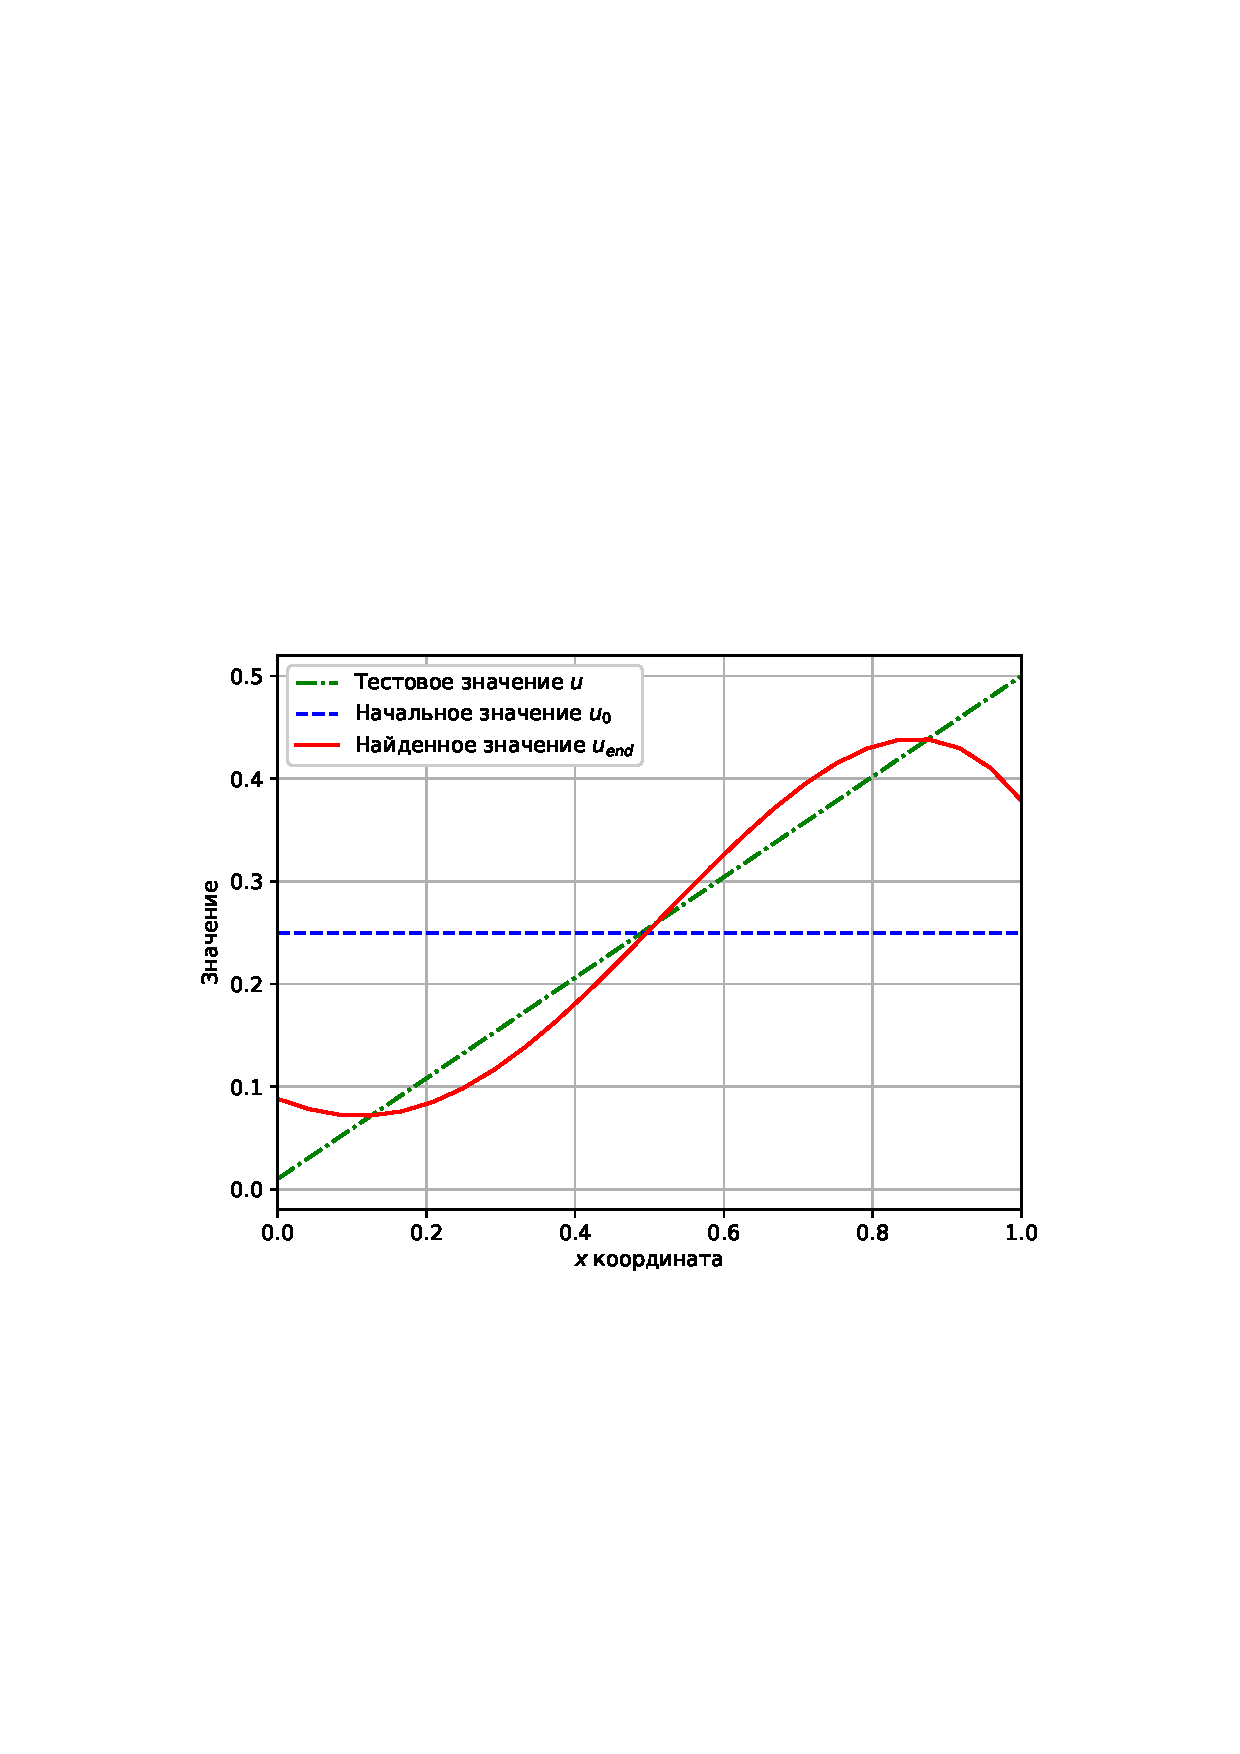
\includegraphics[width=\linewidth]{first/control_initial_optimal_final.png}
  \caption{Control initial optimal and final}
  \label{fig1:control}
\end{figure}


\begin{figure}
  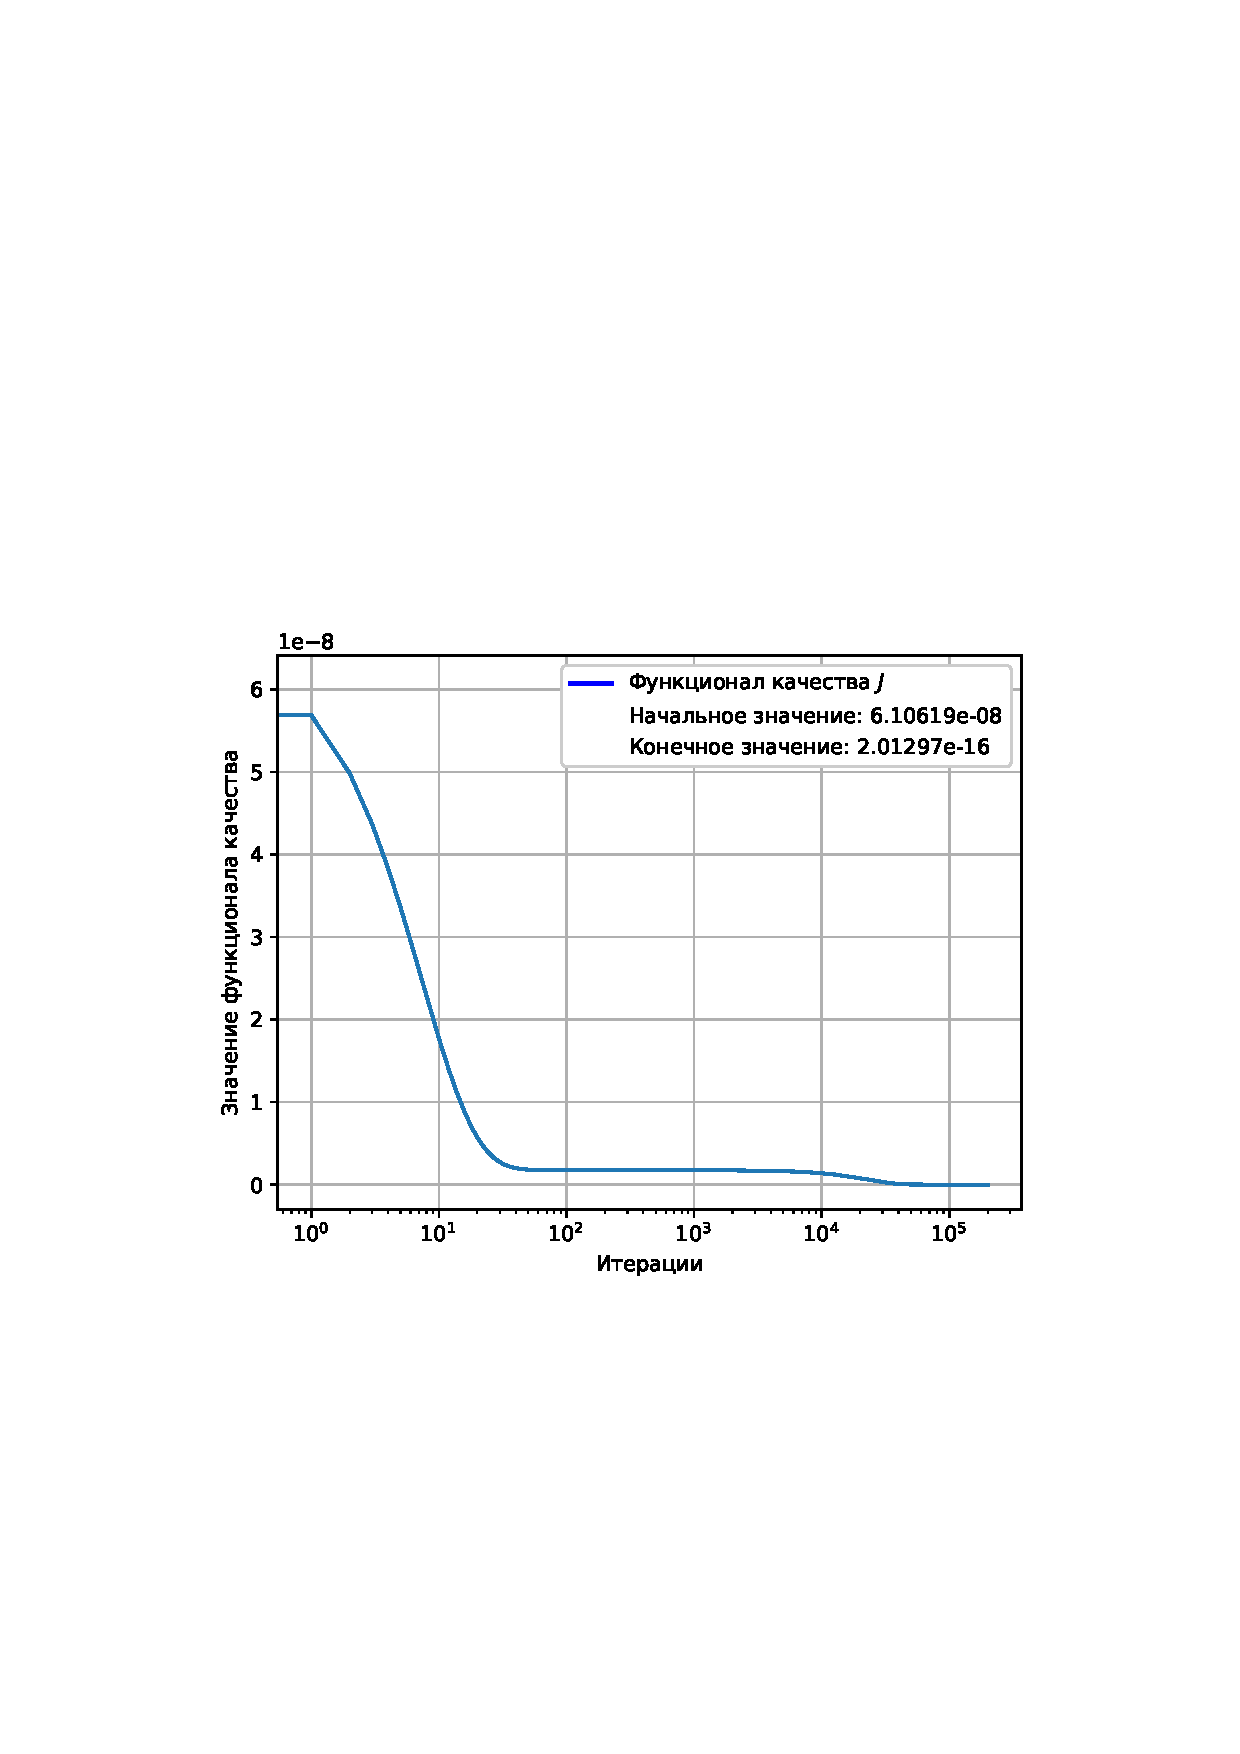
\includegraphics[width=\linewidth]{first/cost_functional_dynamics.png}
  \caption{Функционал качества}
  \label{fig1:cost}
\end{figure}


\begin{figure}
  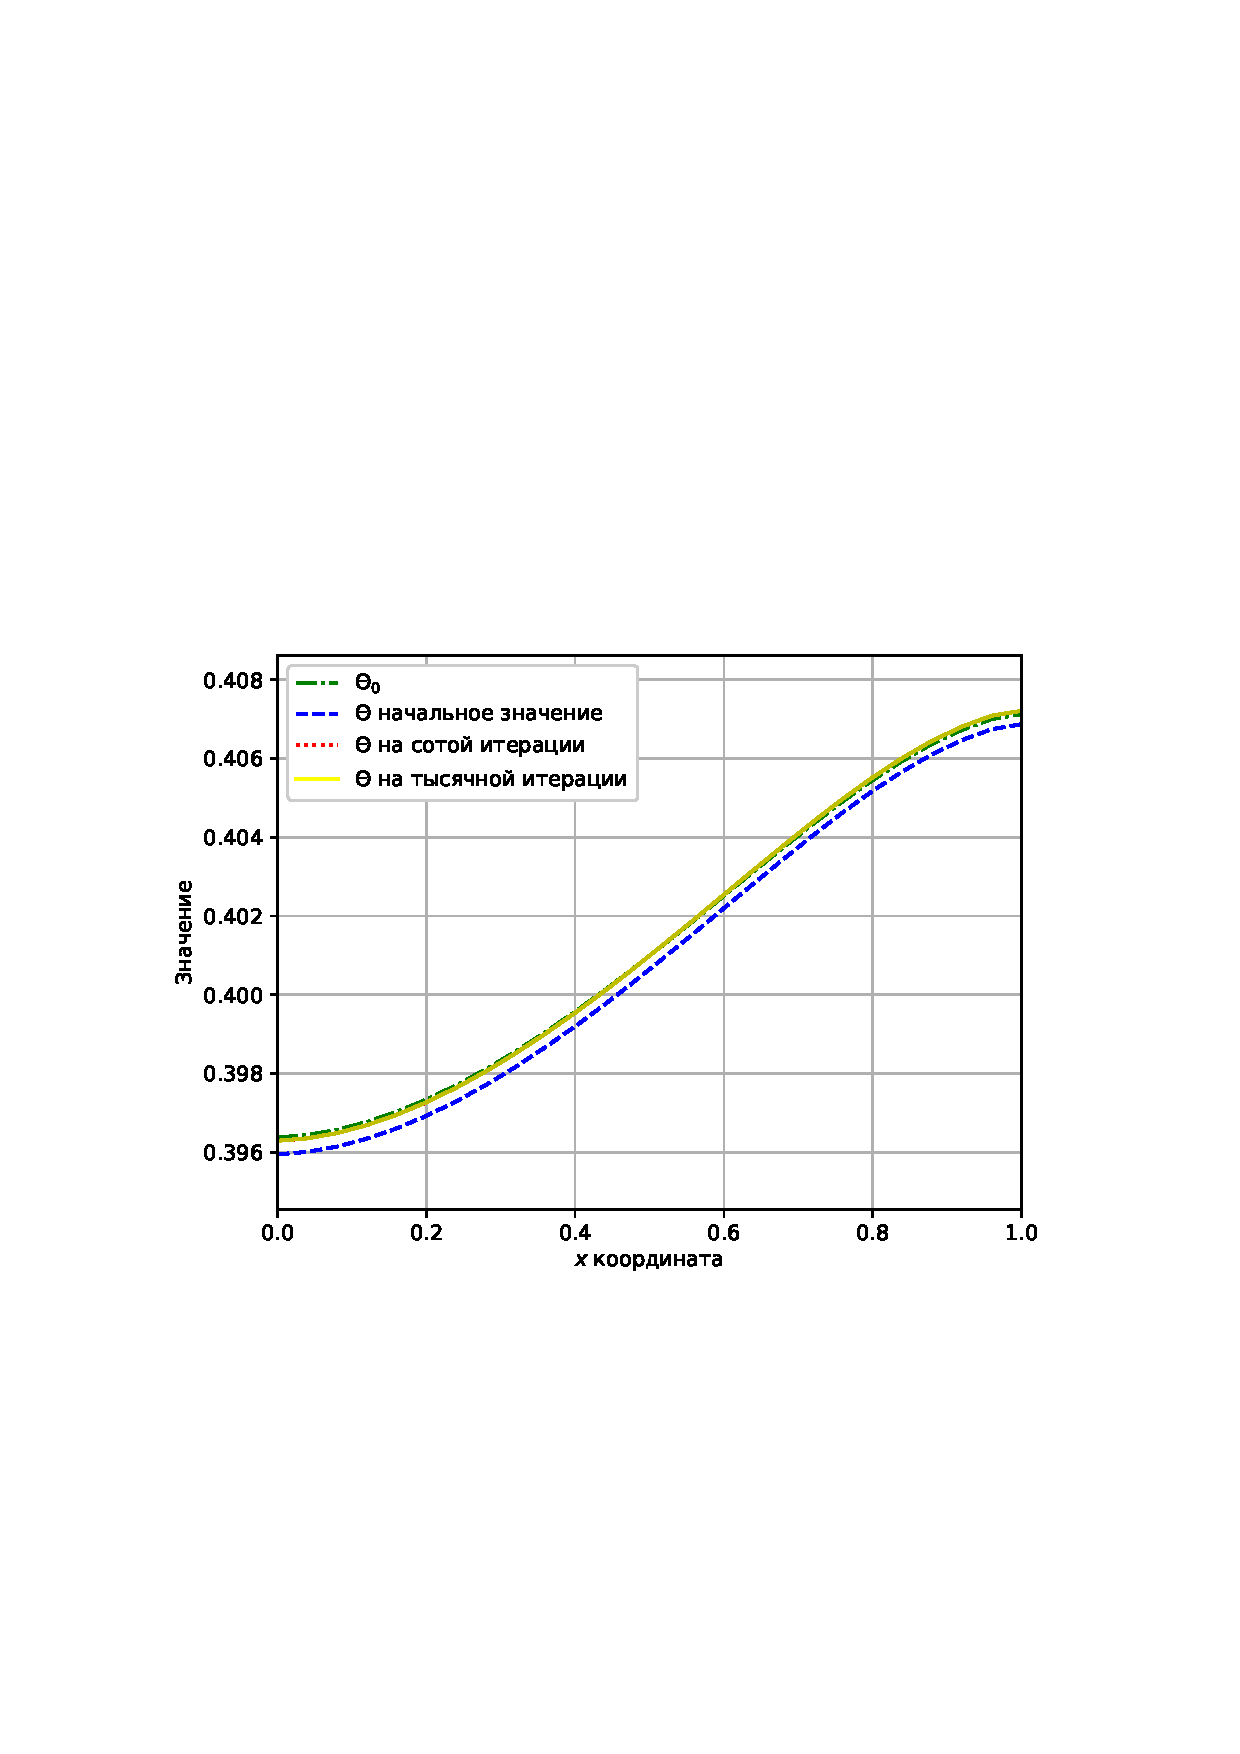
\includegraphics[width=\linewidth]{first/theta_funcs.png}
  \caption{Значения $\theta$ на области контроля}
  \label{fig1:theta}
\end{figure}


\begin{figure}
  \includegraphics[width=\linewidth]{first/theta_optimal.eps}
  \caption{Оптимальное значение $\theta$ в области $\Omega$}
  \label{fig1:cost}
\end{figure}

\begin{figure}
  \includegraphics[width=\linewidth]{first/theta_initial.eps}
  \caption{Начальное значение $\theta$ в области $\Omega$}
  \label{fig1:cost}
\end{figure}

\begin{figure}
  
\includegraphics[width=\linewidth]{first/theta_end.eps}
  \caption{Финальное значение функции $\theta$}
  \label{fig1:cost}
\end{figure}


\newpage



    \bibliographystyle{unsrt}   % this means that the order of references
    			    % is dtermined by the order in which the
    			    % \cite and \nocite commands appear
    \bibliography{bibliography}  % list here all the bibliographies that

\end{document}
